\documentclass{uni_tue_template}

% content of left head area e.g. subject like ETI
\def \headLeft{MatheIII Skript}

% content of center head area, used for names
\def \names{David Morgenstern \& Yannick Runge}

% content of right head area e.g. semester like WiSe 2012/13
\def \headRight{2013/2014}

\newboolean{compileall}
\setboolean{compileall}{false}

\usepackage{hyperref}
\usepackage{multirow}
\usepackage{color}

\title{Mathematik III Prof. Hauck}
\author{David Morgenstern \& Yannick Runge}

\begin{document}
\ifthenelse{\boolean{compileall}}{
	\thispagestyle{empty}
	\maketitle
	\tableofcontents
	\thispagestyle{empty}
	\cleardoublepage
	\setcounter{page}{1}
	\foreach \inputpage in {1,...,9} {
		\input{Math_C\inputpage}
	}
}{
	\newpage
\section{Orthogonale Abbildungen, symmetrische Abbildungen, Kongruenzabbildungen}
\subsection{Definition}
	$ V $ Euklidischer Vektorraum mit Skalarprodukt\\
	$ \alpha:V\rightarrow V $ lineare Abbildung\\
	$ \alpha $ heißt \textbf{orthogonale Abbildung}, d.h. $ (\alpha(v)|\alpha(w))=(v|w) $ für alle $ v,w\in V $.
	
\subsection{Folgerungen}
	\begin{enumerate}
		\item Orthogonale Abbildungen sind \textbf{längentreu}:\\
		$ ||\alpha(v)||=||v|| $ für alle $ v\in V $
		($ ||v||=\sqrt{(v|v)}=\sqrt{(\alpha(v)|\alpha(v))}=||\alpha(v)|| $)
		\item  Orthogonale Abbildungen sind \textbf{winkeltreu}:\\
		$\sphericalangle(v,w)=\sphericalangle(\alpha(v),\alpha(w)$\\
		$ \cos(\varphi)=\frac{(v|w)}{||v||\ ||w|| } $
		\item Orthogonale Abbildung auf endlich dimensionalen Euklidischen Vektorräumen sind bijektiv (nach a): $ \mbox{Kern}(\alpha)=\lrc{\sigma} $)
		\item  $ \alpha $ orthogonal $ \Rightarrow $ $ \alpha^{-1} $ orghogonal.\\
		($ v,w\in V $. Es existieren $ x,y\in V $ mit $ \alpha(x)=v,\alpha(y)=w $, da $ \alpha $ surjektiv).\\
		$( \alpha^{-1}(v)|\alpha^{-1}(w) )= (\alpha^{-1}(\alpha(x))|\alpha^{-1}(\alpha(y)))=(x|y)\ouset{=}{}{\alpha\mbox{\scriptsize orth.}}(\alpha(x)|\alpha(y))=(v|w) $
		\item  $ \alpha,\beta $ orthogonal Abbildung $ \Rightarrow $ $ \alpha\circ\beta $ ist orthogonale Abbildung\\
		$ V $ endlich dimensional, Menge der orthogonalen Abbildungen auf $ V $ bezüglich $ \circ $ bilden eine Gruppe.
	\end{enumerate}

\subsection{Beispiel}
	\begin{enumerate}[a)]
		\item  Drehungen um $ \sigma $ in $ \mr^2 $ sind orthogonale Abbildungen ($ \mr^2 $ mit Standardskalarprodukt)
		\item  $ \varrho $ Spiegelung im $ \mr^2 $ an Achse durch Nullpunkt $ \cdot $ orthogonale Abbildung\\
		$ v_1 $ in Achse, $||v_1||=1$\\
		$ \mathcal{B}=(v_2,v_2) $ ONB\\
		$ A_\varrho^{\mathcal{B}}=\begin{pmatrix}
		1&0\\
		0&-1
		\end{pmatrix}$
	\end{enumerate}
	
\subsection{Satz - Charakteristische orthogonale Abbildung}
	$ V $ $ n $- dim. Euklidischer Vektorraum, $ \mathcal{B}=(v_1,...,v_n) $ ONB von $ V $, $ \alpha: V\rightarrow V $ linear, $ A=A_\alpha^{\mathcal{B}} $. Dann sind äquivalent:
	\begin{enumerate}[(1)]
		\item $ \alpha $ ist orthogonale Abbildung
		\item  $ A\cdot A^t=A^t\cdot A=E_n $\\
		(d.h. $ A^-1=A^t $)
		\item  $ (\alpha(v_1),...,\alpha(v_n)) $ ist ONB
		\item $ ||\alpha(v)||=||v|| $ für alle $ v\in V $
	\end{enumerate}
	
	\textbf{Beweis:}\\
	(1)$ \Rightarrow $(2):\\
	$ A=(a_{ij})_{i,j-1,...,.n} $\\
	$ \varrho_{ij}=(v_i|v_j)=(\alpha(v_i)|\alpha(v_j)=\lrr{\limsum{k=1}{n}a_{ki}\cdot v_k\bigg|\limsum{l=1}{n}a_{lj}v_l} $\\
	$ =\limsum{k.l=1}{n}a_{ki}a_{lj}(v_k|v_l) $\\
	$ =\limsum{k=1}{n}a_{ki}a_{kj} $
	
	$ \Rightarrow A^t\cdot A=E_n $\\
	$ \Rightarrow A^t=A^{-1} $\\
	Daher auch: $ A\cdot A^t=E_n $
	
	(2)$ \Rightarrow $(3):\\
	Wie in (2).\\
	$ A^t\cdot A=E_n\Rightarrow(v_i|v_j)=(\alpha(v_i|\alpha(v_j))) $
	
	(3)$ \Rightarrow $(4):\\
	$ v\in V $, $ v=\limsum{i=1}{n}c_iv_i $\\
	$ \alpha(v)=\limsum{i=1}{n}c_i\alpha(v_i) $\\
	$ (\alpha(v)|\alpha(v))=\limsum{i=1}{n}c_i^2=(u|v) $
	
	(4)$ \Rightarrow $(1):\\
	8.7d): $ (v|w)=\frac{1}{2}(||v+w||^2-||v||^2-||w||^2) $\\
	$ \Rightarrow $ Behauptung
	
\subsection{Definition}
	$ n\times n $- Matrix $ A $ über $ \mr $ heißt \textbf{orthogonale Matrix}, falls $ A\cdot A^t =A^t\cdot A=E_n$\\
	(das bedeutet: Spalten von $ A $ bilden ONB von $ \mr^n $ entsprechenden Zeilen).
	
\subsection{Korollar}
	$ \alpha $ orthogonale Abbildung auf Euklidischem, endlich dimensionalem VRV, $ \mathcal{B} $ ONB von $ V $, $ A=A_\alpha^{\mathcal{B}} $.
	\begin{enumerate}[a)]
		\item $ \det(\alpha)=\det(A)=\pm 1 $
		\item  $ \alpha $ hat höchstens die Eigenwerte $ \pm 1 $ in $ \mr $.
	\end{enumerate}
	
	\textbf{Beweis:}
	\begin{enumerate}[a)]
		\item $ 1\ouset{=}{}{9.4}\det(A\cdot A^t) $\\
		$ \ouset{=}{}{6.7g}\det(A)\cdot\det(A^t) $\\
		$ \ouset{=}{}{6.5}\det(A)^2 $
		\item $ c\in\mr $ Eigenwert von $ \alpha $ $ 0\neq v $ zugehöriger Eigenvektor\\
		$ ||v||=||\alpha(v)||=||c\cdot v||=|c|\cdot||v|| $\\
		$ ||v||\neq 0\quad\Rightarrow\quad |c|=1 $
		
		Orthogonale Abbildungen auf $ \mr^1 $: $ \id, -\id $\\
		Orthogonale Abbildungen auf $ \mr^2 $=
	\end{enumerate}
	
\subsection{Satz}
	$ V $ 2-dim. Euklidischer Vektorraum, $ \mathcal{B}=(v_1,v_2) $ ONB, $ \alpha $ orthogonale Abbildung auf $ V $, $ A=A_\alpha^{\mathcal{B}} $
	\begin{enumerate}[a)]
		\item Ist $ \det(A)=1 $, so ist $ A=\begin{pmatrix}\cos(\varphi)&-\sin(\varphi)\\\sin(\varphi)&\cos(\varphi)\end{pmatrix} $ für ein $ \varphi\in\lra{0,2\pi} $; $ \alpha $ ist Drehung um $ \sigma $ um Winkel $ \varphi $.
			
			\textbf{Bemerkung}

			Ist $V=\mr^2$, und sind $v_1,v_2$ \textbf{positiv orientiert} (d.h. bewegt man sich von $v_1$ nach $v_2$ entgegen des Uhrzeigersinns, dann ist Winkel $\frac{\pi}{2}$), so ist $\alpha$ eine Drehung um den Winkel $\varphi$ entgegen Uhrzeigersinn. Ansonsten Drehung um $\varphi$ im Uhrzeigersinn.
		\item  Ist $ \det(A)=-1 $, so ist $ A=\begin{pmatrix}
		\cos(\varphi)&\sin(\varphi)\\
		\sin(\varphi)&-\cos(\varphi)
		\end{pmatrix} $ für $\varphi\in [0,2\pi[$
		Es gibt ONB $ \varphi=(w_1,w_2) $ mit $ A_\alpha^{\varphi}=\lrv{1&0\\0&1} $. $ \alpha $ ist Spiegelung an Achse $ \lrg{w_1} $.

		\begin{tikzpicture}[scale=1]
			\draw [->] (0,0) -- (3,0) node [anchor=north west] {$ v_1 $};
			\draw [->] (0,0) --(0,3) node [anchor=south east] {$ v_x $};
			\draw [->] (0,0) -- (2,2) node [anchor=west] {$ w_1 $};
			\draw [->] (0,0) -- (-2,2) node [anchor=east] {$ {w_2} $};
			\draw (10mm,0mm) arc (0:45:10mm);
			\draw [dotted] (0,0) -- (-2,-2);
			\draw (0.6,-0.1) node [anchor=south] {$ \frac{\varphi}{2} $};
	 	\end{tikzpicture}

		$w_1$ ist Eigenvektor zum EW1.

		\textbf{Beweis} - WHK, 10.67
	\end{enumerate}

\subsection{Satz}
	Sei $V$ ein dreimentionaler Euklidischer Vektorraum, $\alpha$ orthogonale Abbildung $V\rightarrow V$.\\
	Dann tritt einer der folgenden Fälle ein:
	\begin{enumerate}[a)]
		\item Es existiert ONB $\mathcal{B}=\lrr{v_1,v_2,v_3}$, so dass $A=A_{\alpha}^{\mathcal{B}}=\lrv{\cos\lrr{\varphi}&-\sin\lrr{\varphi}&0\\\sin\lrr{\varphi}&\cos\lrr{\varphi}&0\\0&0&1}$ für ein $\varphi\in [0,2\pi[$\\
			Es ist $\det\lrr{A}=1$
		\item Es existiert ONB $\mathcal{B}=\lrr{v_1,v_2,v_3}$, so dass $A=A_{\alpha}^{\mathcal{B}}=\lrv{\cos\lrr{\varphi}&-\sin\lrr{\varphi}&0\\\sin\lrr{\varphi}&\cos\lrr{\varphi}&0\\0&0&1}$ für ein $\varphi\in [0,2\pi[$\\
			Es ist $\det\lrr{A}=-1$
	\end{enumerate}
	\textbf{Bedeutung}
	\begin{enumerate}[a)]
		\item $\alpha$ ist Drehung um $\varphi$ parallel zur $\lrg{v_1,v_2}$-Ebene mit Drehachse $\lrg{v_3}$
			
		\begin{tikzpicture}
			\draw [->] (0,0) -- (3,0) node [anchor=west] {$ v_2 $};
			\draw [->] (0,0) -- (0,3) node [anchor=south] {$ v_3 $};
			\draw [->] (0,0) -- (-1.5,-1.5) node [anchor=north east] {$ v_1 $};
			\draw [dotted] (0,0) -- (0,-3);
			\draw [->,scale=0.5] (0,0) -- (3,2) node [anchor=west] {$ v $};
			\draw [->,scale=0.5] (0,0) -- (2,3);
			\draw (33.69:10mm) arc (33.69:55.31:10mm);
			\draw [->,green] (33.69:22mm) arc (33.69:55.31:22mm) node [anchor=south] {$ \alpha(v) $};
		\end{tikzpicture}
		
		\item $\alpha$ ist \textbf{Drehspiegelung}:\\
			Drehung um Achse $\lrg{v_3}$ und dann Spiegelung an Ebene $\lrg{v_1,v_2}$
	\end{enumerate}
	\textbf{Spezialfälle}
	\begin{enumerate}[a)]
		\item[Fall a)] $\varphi=0 : \alpha=\id$\\
			$\varphi=\pi: A=\lrv{-1&0&0\\0&-1&0\\0&0&1}$\\
			Achsenspiegelung an $\lrg{v_3}$
		\item[Fall b)] $\varphi=0 : A=\lrv{1&&\\&1&\\&&1}$ - Spiegelung an $\lrg{v_1,v_2}$-Ebene\\
			$\varphi=\pi : A=\lrv{-1&&\\&-1&\\&&-1}$ - Punktspiegelung an $\sigma$
	\end{enumerate}

\subsection{Definition}
	$V$ sei endlich dimensionaler Euklidischer Vektorraum.\\
	Dann heißt die lineare Abbildung $\alpha:V\rightarrow V$ heißt \textbf{symmetrisch} (oder \textbf{selbstadjungiert}), falls gilt $\forall v,w\in V:\;\lrr{v\mid\alpha\lrr{w}}=\lrr{\alpha\lrr{v}\mid w}$

\subsection{Bemerkung}
	Ist $\mathcal{B}$ ONB von $V$, $\alpha:V\rightarrow V$, $A=A_\alpha^{\mathcal{B}}$, so gilt $A=A^t$\\
	Solche Matrizen heißen \textbf{symmetrisch}.

\subsection{Satz von der Hauptachsentransformation}
	\begin{enumerate}[a)]
		\item Ist $\alpha: V\rightarrow V$ symmetrische Abbildung, so existiert \textbf{ONB} $\mathcal{B}$ von $V$, so dass $\mathcal{B}$ aus Eigenvektoren zu $\alpha$ besteht.\\
			$A_\alpha^{\mathcal{B}}=\lrv{c_1&0&0\\0&\ddots&0\\0&0&c_n}, c_i\in\mr$\\
			Insbesondere ist $\alpha$ diagonalisierbar.
		\item Ist $A$ symmetrische Matrix (über $\mr$), dann ex. orthogonale Matrix $B$ mit $B^{-1} A B =B^tAB$ Diagonalmatrix
	\end{enumerate}
	\textbf{Beweis}
	\begin{enumerate}[a)]
		\item WHK 10.75
		\item Vorbemerkung: Ist $A$ irgendeine $n\times n$-Matrix, dann $x,y\in\mr^n$
			
			$\lrr{A\cdot x\mid y} = \lrr{Ax}^t\cdot y = x^t\cdot\lrr{A^t\cdot y}=\lrr{x\mid A^t\cdot y}$\\
			Ist $A=\overline{A^t}$, so ist $\alpha: x\mapsto Ax$ bezüglich des Standardskalarprodukts in $\mr^n$ symmetrische Abbildung\\
			$A=A_\alpha^{\mathcal{B}}, \mathcal{B}$ kanonische Basis

			$\ouset{\Rightarrow}{\smt{a)}}{}$ Es existiert ONB $\mathcal{B}'$ mit $A_\alpha^{\mathcal{B}'}$ Diagonalmatrix.\\
			Basiswechselmatrix $\mathcal{B}\rightarrow\mathcal{B}'$: $B$\\
			$B^{-1}AB=A_\alpha^{\mathcal{B}'}$ Diagonalmatrix
	\end{enumerate}

\subsection{Bemerkung}
	Grund für die Bezeichnungen in 9.11 $\alpha:V\rightarrow V$ symmetrisch\\
	$\exists$ ONB $\mathcal{B}=\lrr{v_1,\dots,v_n}$ mit $\alpha\lrr{v_i}=c_iv_i$\\
	$v=\limsum{i=1}{n} x_iv_i$\\
	$\alpha\lrr{v}=\limsum{i=1}{n} x_i\alpha\lrr{v_i}=\limsum{i=1}{n} c_ix_iv_i$\\
	$\lrr{\alpha\lrr{v}\mid v}=\lrr{\sum c_ix_iv_i\mid\sum x_iv_i}=\limsum{i=1}{n} c_ix_i^2$ (Quadratische Form)

	Finde alle $ \binom{x_1} {x_2}\in\mr^n $ mit $ \limsum{i=1}{n}c_ix_i^2=1 $\\
	Die $ v_i\in\mr $ (9.11) bestimmen die Hauptachsen der Quadrate.\\
	Lösung bilden \textbf{Quadrik}.\\
	$ n=2 $: \textbf{Kegelschnitte}\\
	$ c_1x^2+c_2y^2=1 $\\
	$c_1,c_2>0$. Schreibe : $ c_1=\frac{1}{a^2},\ c_2=\frac{1}{b^2} $\\
	$ \frac{x^2}{a^2}+\frac{y^2}{b^2}=1 $, $ a,b>0 $
	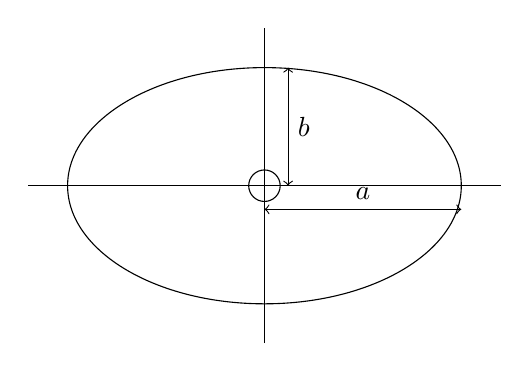
\begin{tikzpicture}
		\draw (-3,0) -- (3,0);
		\draw (0,-2) -- (0,2);
		\draw (0,0) circle (.2cm);
		\draw [<->] (.3,0) -- node [anchor=west] {$b$} (.3,1.5);
		\draw [<->] (0,-.3) -- node [anchor=south] {$a$} (2.5,-.3);
		\draw (0,0) ellipse (25mm and 15mm);
	\end{tikzpicture}

	$c_1>0, c_2<0$ mit $c_1=\frac{1}{a^2}$, $c_2=-\frac{1}{b^2}$ und $a,b>0$\\
	$\frac{x^2}{a^2}-\frac{y^2}{b^2}=1$\\
	$\Rightarrow$ \textbf{Hyperbel}

\subsection{Definition}
	\begin{enumerate}[a)]
		\item Sei $V$ ein $K$-Vektorraum, $b\in V$.\\
			Die Abbildung $t_b:\begin{cases}V\rightarrow V\\v\mapsto v+b\end{cases}$ heißt \textbf{Translation} um $b$.\\
			Nicht linear, falls $b\neq 0$
		\item Kompositionen von linearen Abbildungen und Translationen sind \textbf{affine Abbildungen}.\\
			$\beta\lrr{v}=\lrr{t_b\circ\alpha}\lrr{v}=\alpha\lrr{v}+b$ mit $b\in V$ und $\alpha:V\rightarrow V$ lin. Abb.
		\item $K=\mr$ Affine Abbildungen für die die lineare Abbildung $\alpha$ eine orthogonale Abbildung ist, heißen \textbf{Kongruenzabbildungen}.\\
			$\beta\lrr{v}=\alpha\lrr{v}+b$\\
			Kongruenzabbildungen sind genau die affinen Abbildungen die den Abstand von Vektoren und Winkel unverändert lassen.
	\end{enumerate}
	
\subsection{Bemerkung}
	\begin{enumerate}[a)]
		\item Affine Abbildungen bilden affine Unterräume auf affine Unterräume ab:\\
			$\beta\lrr{v+U}=\alpha\lrr{v}+\alpha\lrr{U}+b =\underbrace{\lrr{\alpha\lrr{v}+b}}_{\in V}+\underbrace{\alpha\lrr{U}}_{\smt{V-UR}}$
		\item Die Hintereinanderausführung von affinen (Kongruenz-) Abbildungen ist wieder affine (Kongruenz-) Abbildung:\\
			$\lrr{\lrr{t_{b'}\circ\alpha'}\circ\lrr{t_b\circ\alpha}}\lrr{v}=\lrr{t_{b'}\circ\alpha'}\lrr{\alpha\lrr{v}+b}=(\underbrace{\alpha'\circ\alpha}_{\ouset{\smt{lin.Abb}}{}{\smt{orth. Abb}}})\lrr{v}+\underbrace{\alpha'\lrr{b}+b'}_{\smt{Trans. Vek.}}$
		\item Affine Abbildungen auf $n$-dimensionalem Vektorraum lass sich nicht durch $n\times n$-Matrizen beschreiben.\\
			Es gibt Darstellungen mit $\lrr{n+1}\times\lrr{n+1}$-Matrzen (Computergrafik, Robotik)\\
			$\mathcal{B}$ Basis von $V$\\
			$\beta=t_b\circ\alpha$ affine Abbildung\\
			$A=A_\alpha^\mathcal{B}, k_\mathcal{B}\lrr{b}=\lrr{b_1\\\vdots\\b_n}$
			
			$\beta\rightarrow\begin{pmatrix}
				A&b\\0\dots 0&1
			\end{pmatrix}$ (Mit $A$ $n\times n$-Matrix)
			
			$\beta'=t_{b'}\circ\alpha', A'=A_{\alpha'}^\mathcal{B}, k_\mathcal{B}\lrr{b'}$
			
			$\beta'\rightarrow\begin{pmatrix}
				A'&k_\mathcal{B}\lrr{b'}\\0\dots 0&1
			\end{pmatrix}$
			
			$\beta'\rightarrow\begin{pmatrix}
				A'&k_\mathcal{B}\lrr{b'}\\0\dots 0&1
			\end{pmatrix}
			\cdot
			\beta\rightarrow\begin{pmatrix}
				A&b\\0\dots 0&1
			\end{pmatrix}\\
			=\begin{pmatrix}
				A'\cdot A&A'\cdot k_\mathcal{B}\lrr{b}+k_\mathcal{B}\lrr{b'}\\0\dots 0&1
			\end{pmatrix}
			=\begin{pmatrix}
				A'\cdot A&k_\mathcal{B}\lrr{\alpha'\lrr{b}+b'}\\0\dots 0&1
			\end{pmatrix}
			\leftarrow \beta'\circ\beta$
			
			Also: Der Hintereinanderausführung affiner Abbildungen entspricht das Produkt der beiden zugehörigen $\lrr{n+1}\times\lrr{n+1}$-Matrizen
		\item Man kann affine Abbildungen $V\rightarrow W$ definieren als $\beta\lrr{v}=\alpha\lrr{v}+w$ $\alpha:V\rightarrow W$ linear $w\in W$
	\end{enumerate}
	
\subsection{Bemerkung}
	Verschiebung von Koordinatensystemen:\\
	In VR. $O,\underbrace{v_1,\dots,v_n}_{\smt{Basis}}$
	
	%TODO - Graphik einfügen
	
	$\mr^n$: Kartesisches Koodinatensystem $O,e_1,\dots,e_n$ (kan. Basis) (Alte Koord.)\\
	NEuer NUllpunkt. $O'=\lrv{b_1\\\dots\\b_n}$ Koordn. bzgl. alten Koordinatensystem.\\
	Im neuen Koordinatensystem mit Ursprung $O',e_1+b,\dots,e_n+b$ hat $O'$ Koordinaten $\lrv{0\\\vdots\\0}$\\
	$Q\in\mr^n$ Koordinaten im alten Koordinatensystem $\lrv{x_1\\\vdots\\x_n}$\\
	Koordinaten im neuen Koordinatensystem $\lrr{x_1-b_1\\\vdots\\x_n-b_n}$\\
	Drehung um Winkel $\varphi$ mit Drehzentrum $O'$:\\
	$Q$ drehen, $n=2$ : $\lrv{\cos\lrr{\varphi}&-\sin\lrr{\varphi}\\\sin\lrr{\varphi}&\cos\lrr{\varphi}}\lrv{x_1-b_1\\x_2-b_2}$ Koordinaten des gedrehten Punktes bezüglich neuem Koordinatensystem\\
	$\underbrace{\lrv{\cos\lrr{\varphi}&-\sin\lrr{\varphi}\\\sin\lrr{\varphi}&\cos\lrr{\varphi}}\lrv{x_1-b_1\\x_2-b_2}}_{\smt{affine Abb.}}+\lrv{b_1\\b_2}$\\
	Koordinatensystem des um $0'$ gedrehten Punktes bezüglich des alten Koordinatensystems\\
	$\lrr{t_b\circ\alpha\circ t_{-b}}\lrv{x_1\\x_2}$
}
\end{document}
